\documentclass[dvipdfmx]{jsarticle}

\title{ブロック落しゲーム(JavaScript)}
\author{Seiichi Nukayama}
\date{2020-06-21}
\usepackage{tcolorbox}
\usepackage{color}
\usepackage{listings, plistings}

% Java
\lstset{% 
  frame=single,
  backgroundcolor={\color[gray]{.9}},
  stringstyle={\ttfamily \color[rgb]{0,0,1}},
  commentstyle={\itshape \color[cmyk]{1,0,1,0}},
  identifierstyle={\ttfamily}, 
  keywordstyle={\ttfamily \color[cmyk]{0,1,0,0}},
  basicstyle={\ttfamily},
  breaklines=true,
  xleftmargin=0zw,
  xrightmargin=0zw,
  framerule=.2pt,
  columns=[l]{fullflexible},
  numbers=left,
  stepnumber=1,
  numberstyle={\scriptsize},
  numbersep=1em,
  language={Java},
  lineskip=-0.5zw,
  morecomment={[s][{\color[cmyk]{1,0,0,0}}]{/**}{*/}},
}
%\usepackage[dvipdfmx]{graphicx}
\usepackage{url}
\usepackage[dvipdfmx]{hyperref}
\usepackage{amsmath, amssymb}
\usepackage{itembkbx}
\usepackage{eclbkbox}	% required for `\breakbox' (yatex added)
\usepackage{setspace}
\usepackage{multicol}
\fboxrule=1pt
\parindent=1em
\begin{document}

%% 修正時刻: Sun Jun 21 08:35:35 2020


\section{壁にぶつかるようにする}

\subsection{画面の各セルの状態を配列で表す}

ブロックが壁にぶつかるようにします。
そのために、通れるセルと通れないセルを数値で表します。
\begin{tcolorbox}
 100 -- 通れるセル \\
  99 -- 壁 \\
  0...6 -- ブロックが積まれているセル
\end{tcolorbox}

そしてそのデータを2次元配列で持ちます。

次のコードをブロックの種類と向きの変数をセットしているところの下に
書き加えてください。

 \begin{lstlisting}[caption=program.js]
  // 画面の各セルの状態
 const joutai = new Array(23);
 \end{lstlisting}

そして、次のコードを ゲーム開始関数gamekaishi() の上に書いてください。
 
\begin{lstlisting}[caption=program.js]
 /**
 * 画面の各セルにデータを埋め込む
 * 100 -- 移動できるセル
 *  99 -- 壁
 *  0...6 -- ブロックが積まれているセル
 */
function setupJoutai() {
  let i, j;

  const joutai = new Array(23);
  for (i = 0; i < 23; i++) {
	joutai[i] = new Array(12);
	for (j = 0; j < 12; j++) {
	  joutai[i][j] = 100;
	}
  }
  // 左壁
  for (i = 0; i < 23; i++) {
	joutai[i][0] = 99;
  }
  // 右壁
  for (i = 0; i < 23; i++) {
	joutai[i][11] = 99;
  }
  // 下壁
  for (j = 0; j < 12; j++) {
	joutai[21][j] = 99;
    joutai[22][j] = 99;
  }
}
\end{lstlisting}

どのようなデータになるのか、表形式で表示してみます。

まず、表示するための場所をHTMLにつくります。

 \begin{lstlisting}[caption=index.html]
  ... (省略) ...
 <button id="kaishibtn" onclick="gamekaishi()">ゲーム<br>スタート</button>
 <div id="joutai-area"></div>
 <footer>
   <small>&copy; 2019 Seiichi Nukayama</small>
  </footer>
  ... (省略) ...
 \end{lstlisting}

 スタイルシートも準備しておきます。

 \begin{lstlisting}[caption=style.css]
  #joutai-area {
    position: absolute;
    top: 150px;
    left: 500px;
    font-size: 0.8em;
  }
 \end{lstlisting}

 printJoutai()関数を書きます。
今記述したsetupJoutai()関数の上に書いてください。

\begin{lstlisting}[caption=program.js]
// 画面の各セルの状態を表示する
function printJoutai() {
  let i, j;
  const joutaiArea = document.getElementById('joutai-area');
  let joutaiHtml;

  joutaiHtml = '<table>';
  for (i = 0; i < 23; i++) {
    joutaiHtml = joutaiHtml + `<tr><th>${i}:</th>`;
	for (j = 0; j < 12; j++) {
      joutaiHtml = `${joutaiHtml}<td>${joutai[i][j]}</td>`;
	}
    joutaiHtml = joutaiHtml + '</tr>';
  }
  joutaiHtml = joutaiHtml + '</table>';

  joutaiArea.innerHTML = joutaiHtml;
}
\end{lstlisting}

\begin{lstlisting}[caption=program.js]
 function gamekaishi() {
   ... (省略) ...
   // 画面を消す
   cg.clearRect(0, 0, 239, 439);

   // 画面データをつくる
   setupJoutai();
   // 画面データを表示
   printJoutai();
  
   ... (省略) ...
 }
\end{lstlisting}

これでブラウザを更新し、ゲームスタートボタンをクリックすると、
以下のような表示になります。

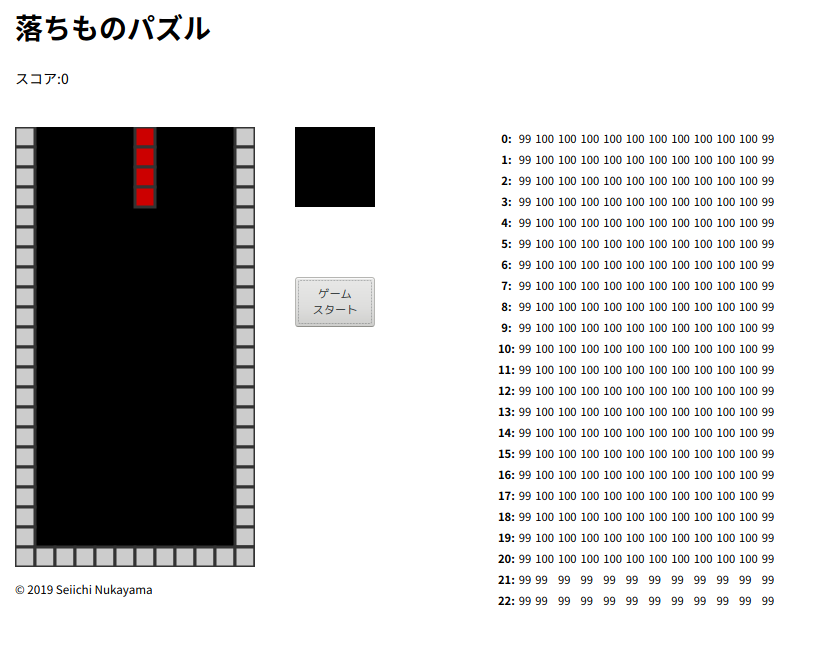
\includegraphics[width=15cm]{game6-2-1.png}

\subsection{ブロックの動きを制限する}

ユーザーが矢印キーを操作すると、それはugokasu()関数で把握しています。
例えば、左キーを押したとき、壁に当たったのかどうかの判定が必要です。
もし、壁じゃなかったら移動が可能ですし、壁だったら移動できません。

そこで、その判定のための関数 kakunin() を作ります。

\begin{lstlisting}
/**
 * kakunin -- 移動回転が可能かどうかを判定する
 * 引数
 *   col -- 現在のx座標(ブロックの左上)
 *   row -- 現在のy座標(ブロックの左上)
 *   syurui -- ブロックの種類(0...6)
 *   muki -- ブロックの向き(0...3)
 * 返り値
 *   true -- 移動は可能
 *   false -- 移動は不可能
 */
function kakunin(col, row, syurui, muki) {
  let x, y;
  let hantei = true;
  const thisBlock = block[syurui][muki];

  for (y = 0; y < 4; y++) {
	for (x = 0; x < 4; x++) {
      if (thisBlock[y][x] === 1) {
        // もしx座標が左の壁にはいったら 
        if (col + x < 1) {
          // x座標を戻す
		  col = col + 1;
		  return false;
		}	
        // もしx座標が右の壁に入ったら
        if (col + x > 11) {
          // x座標を戻す
		  col = col - 1;
		  return false;
        }
        // ブロックのどこかが 100 でなかったら
        // そこは移動可能な場所ではない。
		if (joutai[row + y][col + x] !== 100) {
		  return false;
		}
	  }
	}
  }
  return hantei;
}
\end{lstlisting}

矢印キーでブロックの動きを作っているところで kakunin() を呼び出してチェック
することにします。

\begin{lstlisting}
/**
 * keyCode: left 37  up 38   right 39  down 40
 */
function ugokasu(e) {
  const gamegamen = document.getElementById('game');
  const cv = gamegamen.getContext('2d');	
  let mukiOrg;    // オリジナルの向きを覚えておく
  
  kesu(cv, col, row, syurui, muki);

  switch (e.keyCode) {
  case 37:
    // kakunin()がtrueならcolを左に移動
    if (kakunin(col - 1, row, syurui, muki)) {
      col = col - 1;
      otoKaiten();
    }
	break;
  case 38:
    mukiOrg = muki;
    muki = muki + 1;
    if (muki > 3) {
      muki = 0;
    }
    // もし、回転してkakunin()が false なら
    if (! kakunin(col, row, syurui, muki)) {
      // 向きを元に戻す
      muki = mukiOrg;
    }
	otoKaiten();
	break;
  case 39:
    // kakunin()が true なら colを右に移動
    if (kakunin(col + 1, row, syurui, muki)) {
	  col = col + 1;
      otoKaiten();
    }
    break;
  case 40:
    // kakunin()が true なら row を一つ下に移動
    if (kakunin(col, row + 1, syurui, muki)) {
      row = row + 1;
      otoOchiru();
    }
    // もし kakunin()が false なら、底についたということ
    else {
      kaku(cv, col, row, syurui, muki);
      // 底についた音
      // 次のブロックを表示する
    }
	break;
  }
  kaku(cv, col, row, syurui, muki);
}
\end{lstlisting}

これで壁をすり抜けたり、底を突き抜けたりしなくなりました。

\begin{multicols}{3}
 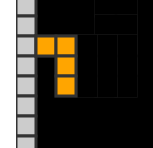
\includegraphics{game7-1.png} \\
 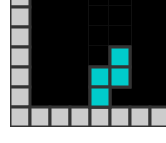
\includegraphics{game7-2.png} \\
 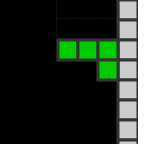
\includegraphics{game7-3.png}
\end{multicols}

底に着いた音を指定しましょう。

以下の記述を otoOchiru() の下に付け加えてください。

\begin{lstlisting}
 function otoDon() {
  document.getElementById('don').play();
}
\end{lstlisting}

そして、矢印キーで下を押したときの処理のところに以下のように書いてください。

 \begin{lstlisting}
  ... (省略) ...
  function ugokasu(e) {
  ... (省略) ...
    case 40:
      // kakunin()が true なら row を一つ下に移動
      if (kakunin(col, row + 1, syurui, muki)) {
        row = row + 1;
        otoOchiru();
      }
      // もし kakunin()が false なら、底についたということ
      else {
        kaku(cv, col, row, syurui, muki);
        otoDon();       // 底についた音              //  <=== ココ
        // 次のブロックを表示する
      }
  }
  ... (省略) ...
 \end{lstlisting}


  \subsection{次のブロックを表示する}

 ブロックが底に着いたとき、次のブロックを表示するのだけれど、その前にやっておく
 ことがあります。
 それは、底に着いたブロックのデータを残しておくことです。 \\
 画面データの配列 joutai[][] を作っているので、それにデータを残します。
 以下のコードを kakunin()関数の下に書いてください。

 \begin{lstlisting}
/**
 * ブロックが底についたときの処理
 * 画面データの配列 joutai[][] の
 * 各セルにそのブロックのsyuruiを埋め込む。
 * syurui -- 0...6
 */
function atBottom(col, row, syurui, muki) {
  const thisBlock = block[syurui][muki];
  let x, y;

  for (y = 0; y < 4; y++) {
    for (x = 0; x < 4; x++) {
      if (thisBlock[y][x] === 1) {
        joutai[row + y][col + x] = syurui;
      }
    }
  }
}
 \end{lstlisting}


 そして、ugokasu()関数の case40: のところの otoDon() を書いたところに
 以下を書いてください。
 \begin{lstlisting}
  ... (省略) ...
  function ugokasu(e) {
    ... (省略) ...
    case 40:
    ... (省略) ...
      else {
      kaku(cv, col, row, syurui, muki);
      otoDon();  // 底についた音
      // 画面データの配列 joutai にブロックの種類を埋め込む
      atBottom(col, row, syurui, muki);
      printJoutai();                            // <=== 確認用
      // 次のブロックを表示する
    } 
  }
 \end{lstlisting}

 このようにブロックの種類が画面データとして記憶されます。

 \begin{multicols}{2}
  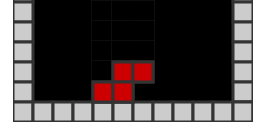
\includegraphics{game7-4.png} \\
  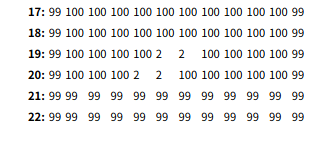
\includegraphics{game7-5.png} 
 \end{multicols}

 さて、次のブロックを表示する処理にとりかかります。\\
 まず、次のブロックを表すオブジェクトを作成します。\\
 joutai という画面データを記憶する配列を定義したところに以下を書き足して
 ください。

 \begin{lstlisting}
  // 画面の各セルのデータ
  const joutai = new Array(23);
  
  // 次のブロック
  const nextBlock = {syurui: 0, muki: 0};
 \end{lstlisting}

 次のブロックに処理の対象を変える関数 changeToNextBlock() を
 書きます。\\
 先ほどの atBottom()関数の下に以下を書き加えてください。

\begin{lstlisting}
 /**
 * 次のブロックに処理を切り変える
 * 次のブロックの情報(種類、向き)は、
 * nextBlock から得る。
 */
function changeToNextBlock() {
  col = Math.floor(Math.random() * 7) + 1;
  row = 0;
  syurui = nextBlock.syurui;
  muki = nextBlock.muki;
}
\end{lstlisting}

これは、次のブロックの種類を向きを乱数を使って決めています。
それから、次のブロックを表示する小窓に次のブロックを表示します。

\begin{lstlisting}
 /**
 * 次のブロックの種類と向きを決定する。
 * 次のブロックを小窓に表示する。
 */
function makeNext() {
  const nextSyurui = Math.floor(Math.random() * 7);
  const nextMuki = Math.floor(Math.random() * 4);
  // 次のブロックを表示する小窓
  const nextGamen = document.getElementById('tsugi');
  const nextCV = nextGamen.getContext('2d');

  // 表示する前に消す
  nextCV.clearRect(0, 0, 79, 79);
  kaku(nextCV, 0, 0, nextSyurui, nextMuki);
  nextBlock.syurui = nextSyurui;
  nextBlock.muki = nextMuki;
}
\end{lstlisting}

これらの関数を ugokasu()関数の switch文の中の \verb!case 40:! で
呼び出します。\\
先ほどの atBottom(), printJoutai() の後に書いてください。

\begin{lstlisting}
  // 画面データの配列 joutai にブロックの種類を埋め込む
  atBottom(col, row, syurui, muki);
  printJoutai();
  changeToNextBlock();           // <== 
  makeNext();                    // <==
\end{lstlisting}

また、gamekaishi()関数にも makeNext() を書き加えてください。

\begin{lstlisting}
function gamekaishi() {
 ... (省略) ...
 
  kaku(cg, col, row, syurui, muki);

  makeNext();                         // <===
} 
\end{lstlisting}


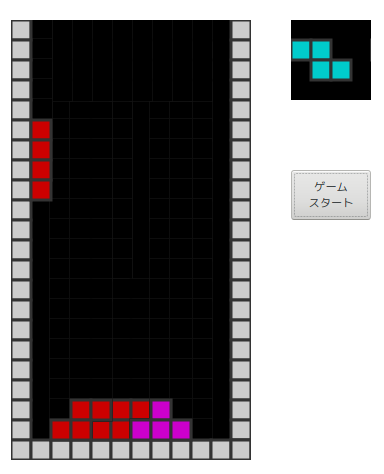
\includegraphics[width=8cm]{game7-6.png}

\end{document}

%% 修正時刻: Sat May  2 15:10:04 2020


%% 修正時刻: Sun Jun 21 19:12:34 2020
